\documentclass[]{article}
\usepackage{geometry}
\geometry{
a4paper,
total={170mm,257mm},
left=20mm,
top=20mm,
}
\usepackage{booktabs} 
\usepackage{longtable}
\usepackage{appendix}
\usepackage{graphicx}
\usepackage{subcaption}
\usepackage{listings}
\usepackage[justification=centering]{caption}
\usepackage{hyperref}
\usepackage{enumitem}
\usepackage[utf8]{inputenc}
\usepackage{float}
\DeclareTextFontCommand{\helvetica}{\fontfamily{phv}\selectfont}
\setlength{\parindent}{4em}
\setlength{\parskip}{1em}
\linespread{1.5}

\usepackage[table]{xcolor}
\usepackage{graphicx}
\usepackage{adjustbox}

\title{Memoria del treball final de màster}
\date{15 d'Abril 2019}
\author{Vasyl Druchkiv \\ Estudiant del Màster de Bioestadística i Bioinformàtica}
\renewcommand{\contentsname}{Índice}
\usepackage{setspace}


\renewcommand\paragraph{\@startsection{paragraph}{4}{\z@}%
{-2.5ex\@plus -1ex \@minus -.25ex}%
{1.25ex \@plus .25ex}%
{\normalfont\normalsize\bfseries}}

\begin{document}
\maketitle
\makeatletter

\makeatother
\begin{spacing}{0.1}
\tableofcontents
\end{spacing}

\begin{center}
\noindent\rule{8cm}{0.4pt}
\end{center}

\section{Introducció}

\begin{figure}[H]
\centering
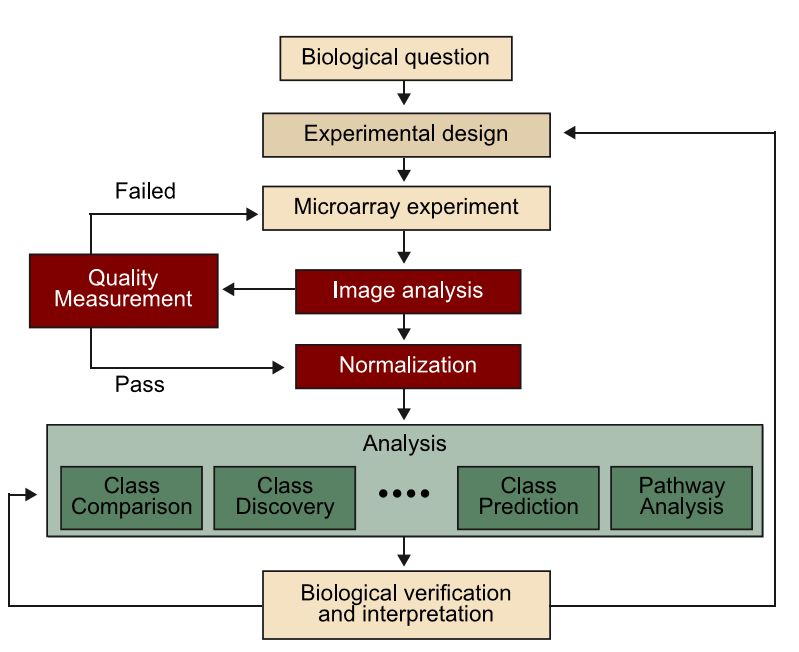
\includegraphics[width=0.9\textwidth]{Pipeline_Microarray.jpg} 
\caption{El procès d'anàlisi de microarrays}
\end{figure}

\section{Descripció dels mètodes} 

\section{Anàlisi de les rutes - final del pipeline d'anàlisi d'expressió}


\begin{figure}[H]
\centering
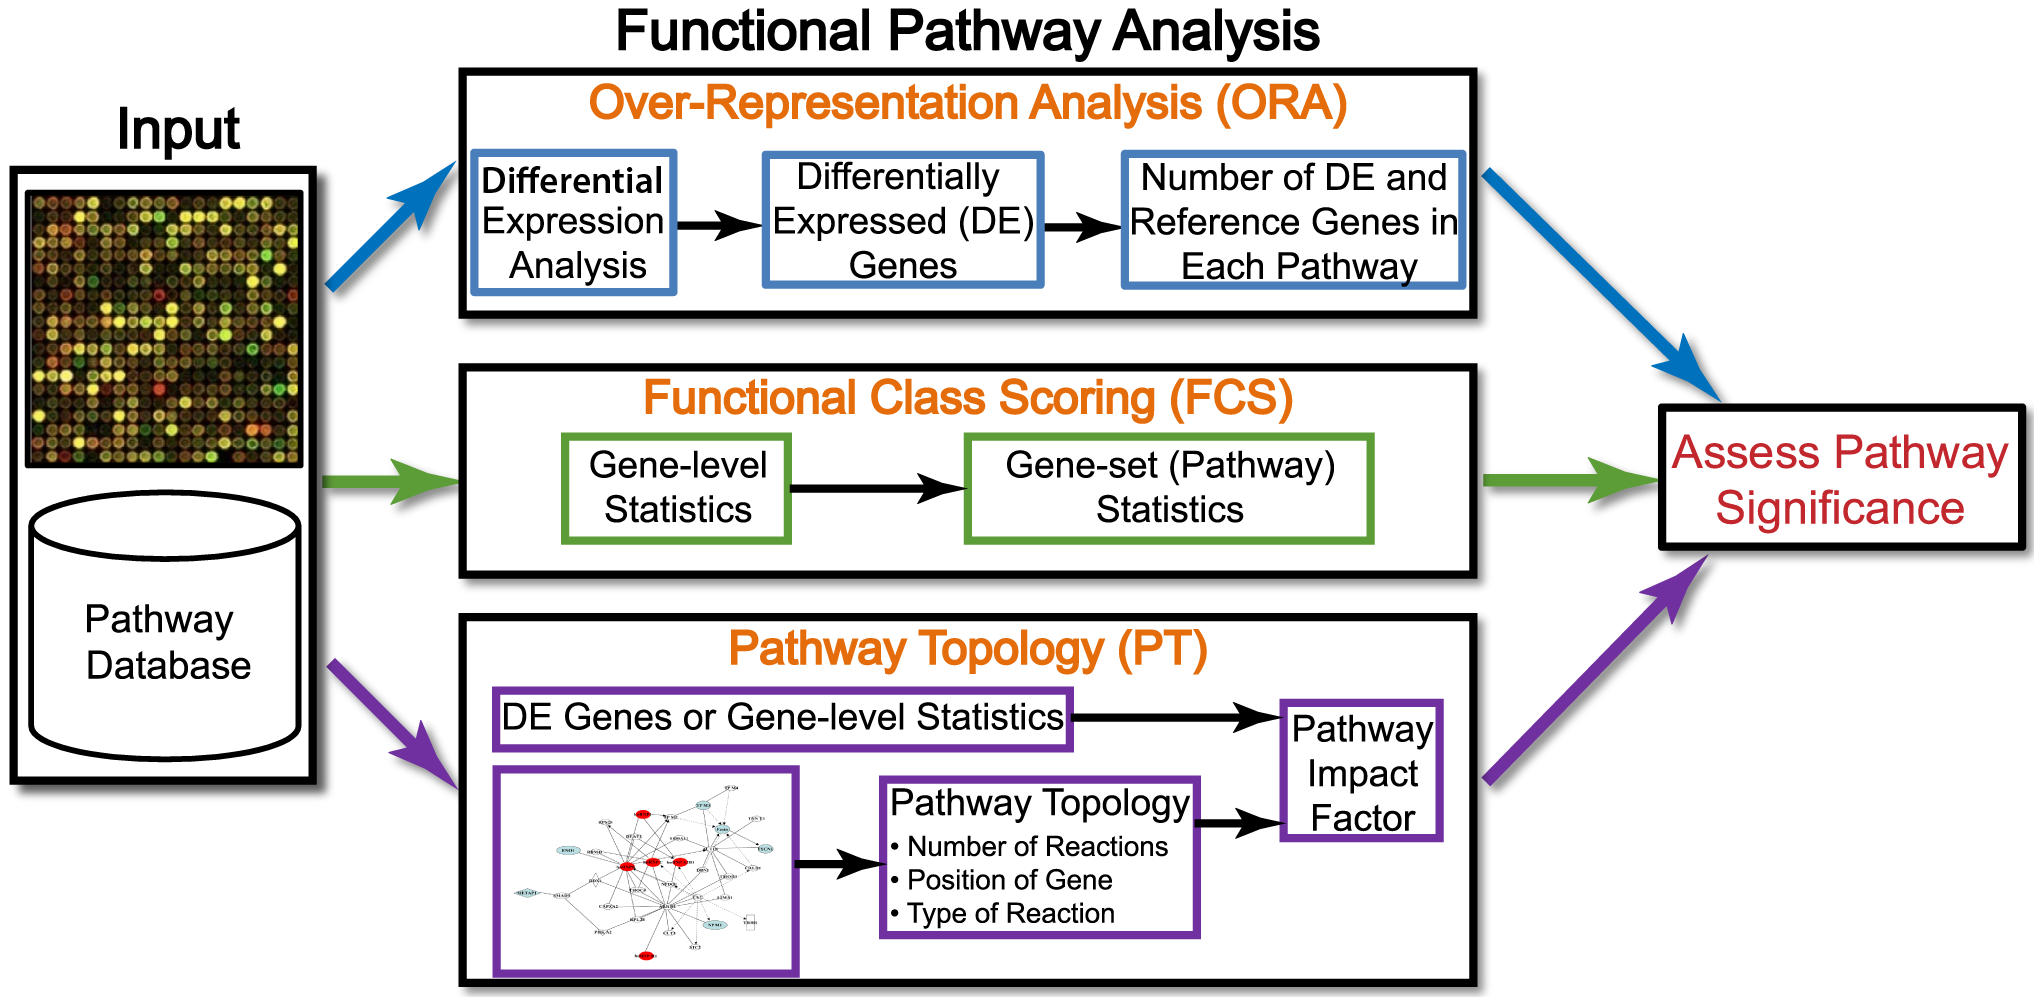
\includegraphics[width=0.9\textwidth]{Pipeline_Pathway.png} 
\caption{El procès d'anàlisi de les rutes}
\end{figure}



\subsection{ORA}

L'anàlisi de sobreexpressió és una tècnica d'identificació de les rutes significativament enriquides en la mostra d'interès. 

El paper original què se cita habitualment quan es parla d'anàlisi d'expressió genètica és de \cite{boyle2004go}. El mètode estadístic descrit consisteix bàsicament en els pasos següents:

\begin{enumerate}
\item \textbf{De tots els gens de la mostra seleccionar un grup de gens que es considera que són significativament expressats.}

Els criteris de selecció poden baser-se en \textit{log ratios} o/i en el valor de p provenent d'un test estadístic. \textit{Log ratios} donen la magnitut amb el qual un gen és sobre o sotaexpressats. Les diferències entre els grups però són el resultat d'un procès estochàstic i per tan hem d'intentar de minimitzar el risc de prendre decisions falses. El valor de p representa la probabilitat d'aquest risc i per tant dona certa confiança sobre la significació de les diferències observades.

\item \textbf{Determinar si algunes rutes anoten la llista especificada de gens amb la freqüència més alta que un esperaria per casualitat.} 

El test estadístic es basa en la distribució hipergeomètrica: 

$$p = 1 - \displaystyle\sum_{i = 0}^{k-1}\frac{{M \choose i}{{N-M} \choose {n-i}}} {{N \choose n}}$$

En aquesta equació $N$ és el nombre total de gens en la distribució de fons, $M$ és el nombre de gens dins d'aquesta distribució que són anotats a la ruta d'interès, $n$ és el nombre total en la llista especificada de gens i $k$ és el nombre de gens dins d'aquesta llista que són anotats a la ruta. La distribució de fons pot ser o bé tots els gens en la base de dades d'anotació o bé tots els gens d'experiment.

El valor de P obtingut amb aquesta formula dona la probabilitat de veure el nombre $x$ de gens de la llista relacionats amb la ruta específica en la llista del nombre total de gens $n$ donat la proporció de gens relacionats amb aquesta ruta en la distibucó de fons.
 
\end{enumerate}

L'aplicació utilitza aquesta idea i calcula una taula amb els camps següents:


\begin{itemize}
\item \underline{Description}. El nom del terme GO;
\item \underline{GeneRatio}. El quocient: $\displaystyle\frac{\mbox{Nombre dels gens diferencialment expressats que pertanyen al conjunt de gens}}{\mbox{Nombre total dels gens diferencialment expressats}}=\frac{M}{N}$; 
\item \underline{BgRatio}. El quocient: $\displaystyle\frac{\mbox{Nombre dels gens del conjunt d'interès en la distribució de fons}}{\mbox{Nombre total dels gens en la distribució de fons}}=\frac{k}{n}$;
\item \underline{pvalue}. Valor de p basat en la distribució hipergeomètrica descrita anteriorment.
\item \underline{p.adjust}. El valor de P ajustat. L'usuari pot seleccionar el mètode d'ajustmanent.
\end{itemize}


\subsection{GSEA}

Amb l'anàlisi GSEA podem analitzar els resultats d'un experiment d'expressió per a dos grups. Aquí els gens son ordenats basant-se en la correlació entre la seva expressió i la separació  entre les classes. Aquest llistat ordenat $L$ el podem crear utilitzant els \textit{logRatios}.

Donat el conjunt definit dels gens $S$, que pertanyen per exemple al mateix terme de Gene Ontology, l'objectiu de GSEA és determinar si els membres de $S$ són distribuits aleatoriament en el $L$ o es troben més al cap o a la cua. S'esperaria que els gens relacionats a la separació fenotípica mostraran aquesta última distribució. 

L'anàlisi GSEA consisteix en tres pasos:

\begin{enumerate}
\item Calculació del puntuació d'enriquement (\textit{ES: Enrichment Score}). La puntuació està calculada anant per la llista i augmentant la suma corrent sempre quan es troba un gen que pertany a $S$ o, al contrari, restant-hi quan el gen no forma part del conjunt $S$. La puntuació és la desviació màxima del zero observada en aquet camí. L'estadística obtinguda és la estadística de Kolmogorov-Smirnov amb pesos.

\item Estimació del nivell de significació per a la puntuació \textit{ES}. El valor de P nominal es pot obtenir mitjançant o bé la permutació de les classes o bé la permutació de gens, on l'estadística \textit{ES} observada es compara amb la distribució obtinguda amb permutació. A l'aplicació es fa ús de l'útima opció.
 
 \item Calculació del valor de P ajustat. El valor de P nominal s'ajusta per controlar l'error global que es produeix com a resultat de les comparacions múltiples.
\end{enumerate}

\begin{figure}[H]
\centering
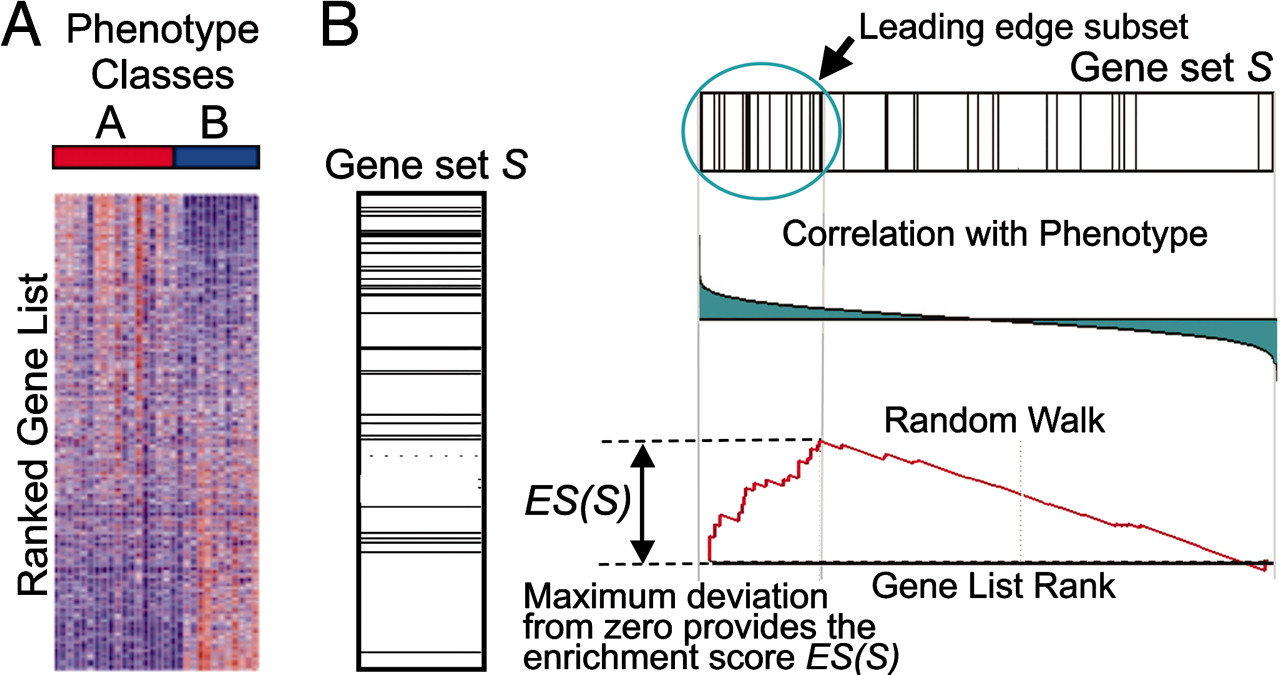
\includegraphics[width=0.9\textwidth]{GSEA_Method.jpg} 
\caption{El mètode GSEA}
\end{figure}

L'aplicació que he desarrolat agafa aquesta idea i calcula la tabla que inclou l'estadístiques següents:

\begin{itemize}
\item \underline{enrichmentScore}. Enrichment score per al conjunt dels gens. Amb altres paraules: el grau amb el qual el conjunt dels gens està sobreexpressat a dalt o a baix del llistat ordenat dels gens en les dades d'expressió.
\item \underline{NES}. Normalized enrichment score. La puntuació per al conjunt de gens després de ser normalitzat tenint en compte tots els conjunts de gens analitzats (la seva mida i la seva correlació amb les dades d'expressió). Aquesta puntuació ajuda a comparar els resultats entre els conjunts de gens.
\item \underline{pvalue}.El valor de p nominal.
\item \underline{p.adjust}. El valor de p ajustat.
\item \underline{leading\_edge}
\begin{itemize}
\item \underline{Tags}. El percentatge de les ocurrències de gens del conjunt específic abans (per als ES positius) o després (per als ES negatius) del cim en la puntuació corrent d'enriquiment. Aquest valor indica el percentatge dels gens que contribueixen a la puntuació d'enriquement. 
\item \underline{List}. El percentatge dels gens en el llistat ordenat de tots els gens abans o després del pic en la puntuació corrent d'enriquiment. Aquest valor ens indica on exactament el pic es produeix. 
\item \underline{Signal}. La fortalesa del senyal d'enriquiment que combina els dos valors anteriors.
\end{itemize}
\item \underline{rank}. La posició del pic en la llista ordenada dels gens. Els conjunts dels gens més interessants assoleixen el seu màxim o bé al principi o al final de la llista ordenada. Vol dir que tenen aquest valor o bé molt baix o bé molt alt.
\end{itemize}

\section{Instalació}

Es pot installar l'aplicació localment utilitzan l'ordre següent de R:

\begin{lstlisting}[language=R]
devtools::install_github("vdruchkiv/TFM/5_Packages/PathwayApp/PathwayApp")
\end{lstlisting}


\section*{Biblilografia}
\addcontentsline{toc}{section}{Biblilografia}
\renewcommand{\section}[2]{}%
%\renewcommand{\chapter}[2]{}% for other classes
\bibliography{references}
\bibliographystyle{apalike}


\end{document}


